\chapter{模板}

\begin{lstlisting}[language={[ANSI]C},
        numbers=left,
        numberstyle=\tiny,
        basicstyle=\small\ttfamily,
        stringstyle=\color{purple},
        keywordstyle=\color{blue}\bfseries,
        commentstyle=\color{olive},
        directivestyle=\color{blue},
        frame=shadowbox,
        %framerule=0pt,
        %backgroundcolor=\color{pink},
        rulesepcolor=\color{red!20!green!20!blue!20}
        %rulesepcolor=\color{brown}
        %xleftmargin=2em,xrightmargin=2em,aboveskip=1em
        ]
int main(int argc, char ** argv)
{
	printf("Hello world!\n");
	return 0;
}



\end{lstlisting}


\begin{lstlisting}[language={[ANSI]C},
        basicstyle=\tiny\ttfamily,
        stringstyle=\color{purple},
        keywordstyle=\color{blue}\bfseries,
        commentstyle=\color{olive},
        directivestyle=\color{blue},
        frame=shadowbox,
        %framerule=0pt,
        %backgroundcolor=\color{pink},
        rulesepcolor=\color{red!20!green!20!blue!20}
        %rulesepcolor=\color{brown}
        %xleftmargin=2em,xrightmargin=2em,aboveskip=0em
        ]
\end{lstlisting}




\begin{figure}[htbp]
\centering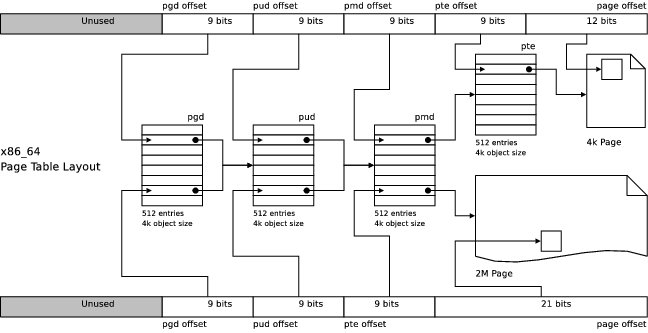
\includegraphics[width=0.9\textwidth]{va-to-pa.png}
\caption{虚拟地址转换}\label{fig:1}
\end{figure}